\documentclass[aps,prb,twocolumn,superscriptaddress,floatfix,longbibliography,nofootinbib]{revtex4-2}

\usepackage{minted, xcolor, graphicx, caption, geometry}
\usepackage{amsmath,amssymb} % math symbols
\usepackage{bm} % bold math font
\usepackage{graphicx} % for figures
\usepackage{comment} % allows block comments
%\usepackage{ulem} % allows strikeout text, e.g. \sout{text}
\usepackage[francais]{babel}

\usepackage{datetime2}

% Redéfinir la commande \today pour supprimer "Dated: "
% \renewcommand{\today}{\DTMdisplaydate{ \the\year}{\the\month}{\the\day}{-1}}
% \newcommand{\ajd}{\DTMdisplaydate{\the\year}{\the\month}{\the\day}{-1}}

% \usepackage[T1]{fontenc}
% \usepackage{lmodern}

\usepackage{float} % allows H in figure placement

\usepackage{minted} % allows colored code
\usepackage{textcomp} % This package gives the text quote '
\usepackage{gensymb} % This package gives the degree symbol \degree

\usepackage{enumitem}
\setlist{noitemsep,leftmargin=*,topsep=0pt,parsep=0pt}


% \usepackage[symbol]{footmisc}
\usepackage{changepage} 

\usepackage{booktabs} 
\usepackage{multirow}

\usepackage{xcolor} % \textcolor{red}{text} will be red for notes
\definecolor{lightgray}{gray}{0.6}
\definecolor{medgray}{gray}{0.4}

\usepackage{hyperref}
\hypersetup{
colorlinks=true,
urlcolor= blue,
citecolor=blue,
linkcolor= blue,
% bookmarks=true,
% bookmarksopen=false,
}


% Code to add paragraph numbers and titles
\newif\ifptitle
\newif\ifpnumber
\newcounter{para}
\newcommand\ptitle[1]{\par\refstepcounter{para}
{\ifpnumber{\noindent\textcolor{lightgray}{\textbf{\thepara}}\indent}\fi}
{\ifptitle{\textbf{[{#1}]}}\fi}}
\ptitletrue  % comment this line to hide paragraph titles
\pnumbertrue  % comment this line to hide paragraph numbers

% minimum font size for figures
\newcommand{\minfont}{6}

% Uncomment this line if you prefer your vectors to appear as bold letters.
% By default they will appear with arrows over them.
\renewcommand{\vec}[1]{\bm{#1}}

% Allows to rewrite the same title in the supplement
\newcommand{\mytitle}{MAC address anonymization}

\begin{document}

% Ajustement des marges
\newgeometry{left=2cm, right=2cm, top=3cm, bottom=3cm}

\title{\mytitle}

% \author{Mickael Kovel, Hugo Charels}
\author{Mickael Kovel}
\affiliation{MA1 Cybersecurity, Université Libre de Bruxelles (ULB), Bruxelles, Belgique}

\date{\today}
% \date{}

\begin{abstract}

    % bla bla bla

\end{abstract}

\maketitle
% \tableofcontents
\section{\label{sec:Intro}Introduction}
bla bla bla

\section{\label{sec:Whatis}What is a MAC address?}
  % In the context of networking, we need to identify devices on a network.
  % en effet, pour echanger des informations entre deux appareils, nous pointons 
  % vers un identifiant. 
  % Dans le contexte d'internet, nous utilisons des adresses IP pour identifier
  % les appareils. Cependant, les adresses IP sont dynamiques et peuvent changer
  % à chaque fois que l'appareil se connecte au réseau.
  % C'est pourquoi nous utilisons des adresses MAC pour identifier les appareils
  % de manière unique, de la même manière que nous utilisons des adresses postales
  % pour identifier les maisons et envoyer du courrier.
  % En anglais:
  In the context of networking, we need to identify devices on a network.
  To exchange information between two devices, we point to an identifier.
  In the context of the internet, we use IP addresses to identify devices.
  However, IP addresses are dynamic and can change each time the device connects to the network.
  This is why we use MAC addresses to uniquely identify devices, in the same way 
  that we use postal addresses to identify houses and send mail.

  We can define a MAC address as a unique identifier assigned to a network interface 
  controller (NIC) for use as a network address in communications within a network segment.

  \subsection{\label{sec:Provided}How is a MAC address provided?}
  MAC addresses are provided by the manufacturer of the network interface controller (NIC).
  They are typically assigned at the factory and are hardcoded into the hardware.
  They cannot be changed by the user and are globally unique.
    \subsubsection{\label{sec:Structure}What is the structure of a MAC address?}
    A MAC address is a 48-bit number that is typically represented as a 12-digit hexadecimal number.
    The first 24 bits (6 digits) are the Organizationally Unique Identifier (OUI), 
    which identifies the manufacturer of the NIC.
    The last 24 bits (6 digits) are the device identifier, which is assigned by the manufacturer.
    The OUI is assigned by the Institute of Electrical and Electronics Engineers (IEEE)
    and is unique to each manufacturer.
    The device identifier is unique to each device and is assigned by the manufacturer.
  \begin{figure}[H]
      \centering
      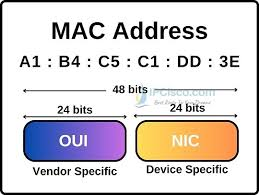
\includegraphics[width=0.5\textwidth]{pictures/mac.jpeg}
      \caption{MAC address structure \cite{MAC}}
      \label{fig:MAC}
  \end{figure}

  \subsection{\label{sec:Privacy}What are the privacy implications of a MAC address?}
  \subsection{\label{sec:Where}Where are MAC addresses used?}
    % \subsubsection{\label{subsec:Network}Network}
    \subsubsection{\label{subsec:Wi-Fi}Wi-Fi - Ethernet}
  % Dans le contexte des réseaux informatiques, les adresses MAC sont utilisées
  % pour identifier les appareils sur un réseau local.
  % Elles sont liées à l'adresse IP d'un appareil et sont utilisées pour acheminer
  % les paquets de données vers la bonne destination.
  % Le protocole ARP (Address Resolution Protocol) est utilisé pour associer une
  % adresse IP à une adresse MAC.
  % En anglais:
  In the context of computer networks, MAC addresses are used to identify devices on a local network.
  They are linked to the IP address of a device and are used to route data packets to the correct destination.
  The Address Resolution Protocol (ARP) is used to associate an IP address with a MAC address.

  \begin{figure}[H]
      \centering
      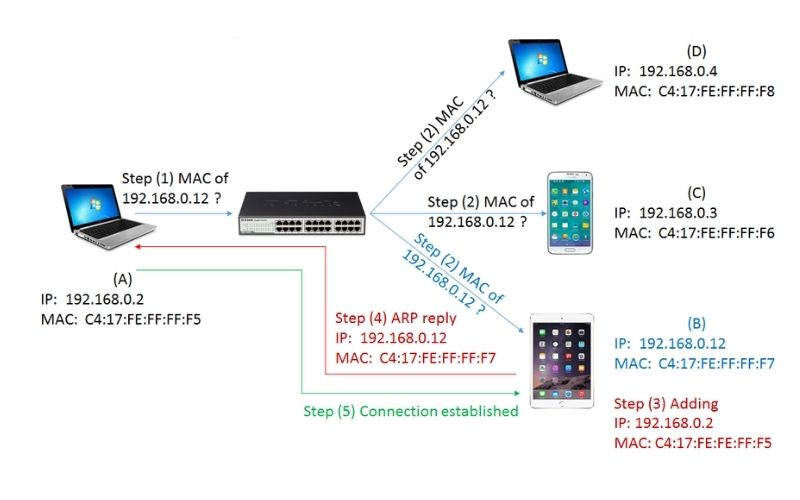
\includegraphics[width=0.5\textwidth]{pictures/arp.jpg}
      \caption{ARP protocol \cite{ARP}}
      \label{fig:ARP}
  \end{figure}
  We can see in the figure \ref{fig:ARP} that the MAC address is used to identify the device in the network.



    % ARP
    \subsubsection{\label{subsec:Bluetooth}Bluetooth}
    Bluetooth devices do not use MAC addresses in the same way as Wi-Fi devices.
    Instead, they use a 48-bit Bluetooth device address (BD\_ADDR) that is similar to a MAC address.
    BD\_ADDRs are also globally unique and could be used to track devices in the same way as MAC addresses.
    \begin{figure}[H]
        \centering
        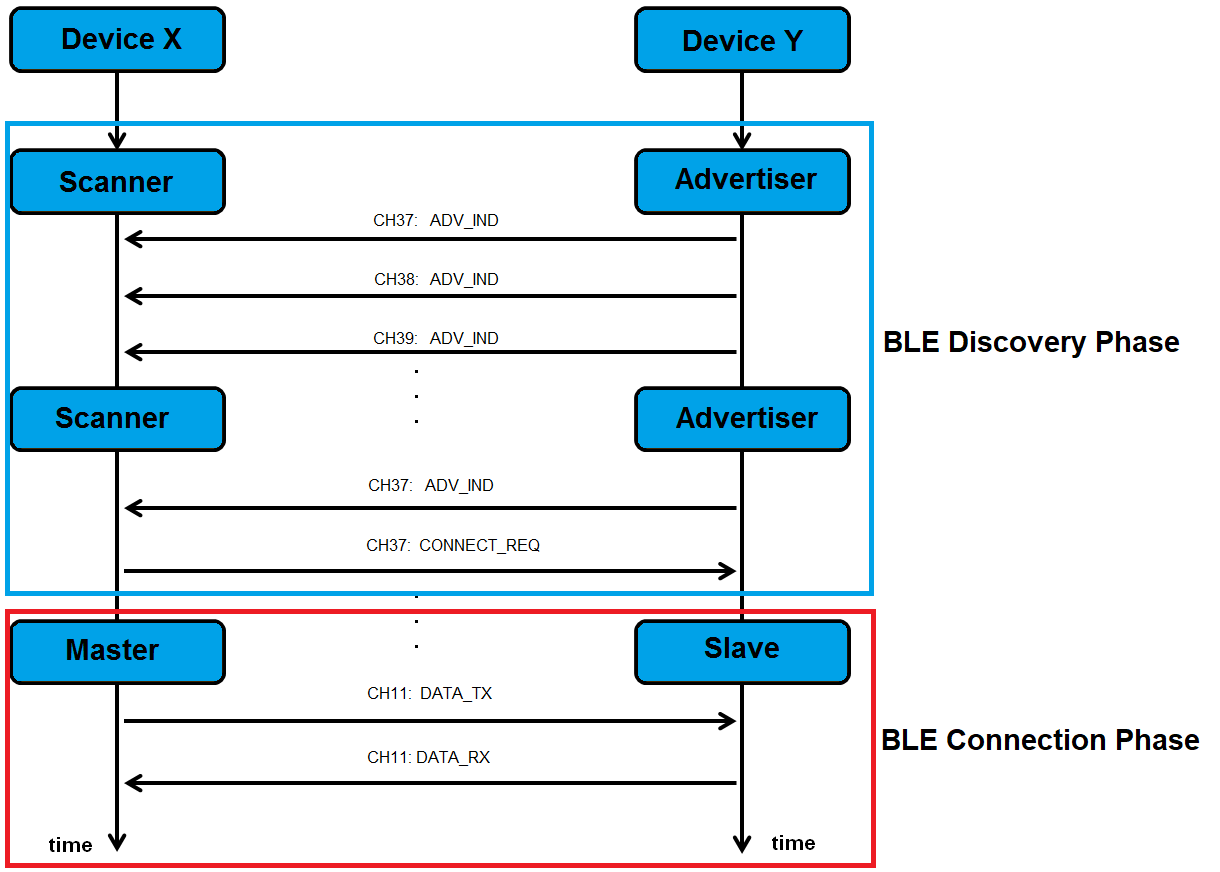
\includegraphics[width=0.5\textwidth]{pictures/Link-Layer-Roles-Change_ver1.png}
        \caption{BTLE Link Layer \cite{BLE5}}
        \label{fig:BT}
    \end{figure}
    We can see in the figure \ref{fig:BT} that even during the discovery phase, there
    is exchange in both directions, which means that the BT\_ADDR have already been 
    exchanged before even connecting to the device.


\section{\label{sec:Law}What does the law say ?}
  \subsection{\label{subsec:GDPR}GDPR}
  The principles of data protection should apply to any information concerning an
  identified or identifiable natural person. 
  Personal data which have undergone pseudonymisation, which could be attributed to a natural person by
  the use of additional information should be considered to be information on an identifiable natural person. To
  determine whether a natural person is identifiable, account should be taken of all the means reasonably likely to
  be used, such as singling out, either by the controller or by another person to identify the natural person directly
  or indirectly. To ascertain whether means are reasonably likely to be used to identify the natural person, account
  should be taken of all objective factors, such as the costs of and the amount of time required for identification,
  taking into consideration the available technology at the time of the processing and technological developments.
  The principles of data protection should therefore not apply to anonymous information, namely information
  which does not relate to an identified or identifiable natural person or to personal data rendered anonymous in
  such a manner that the data subject is not or no longer identifiable. This Regulation does not therefore concern
  the processing of such anonymous information, including for statistical or research purposes.\cite{GDPR2016}

  \subsection{\label{subsec:ECHR}European Convention on Human Rights}
  \begin{enumerate}
    \item[34.] Individual applications
  The Court may receive applications from any person, non-
  governmental organisation or group of individuals claiming to be
  the victim of a violation by one of the High Contracting Parties of
  the rights set forth in the Convention or the Protocols thereto. The
  High Contracting Parties undertake not to hinder in any way the
  effective exercise of this right.

\item[35.] Admissibility criteria
\end{enumerate}
  \begin{enumerate}
    \item[1.] [...]
    \item[2.] The Court shall not deal with any application submitted under Article 34 that
    \begin{enumerate}
      \item is anonymous; or [...]
    \end{enumerate}
  \end{enumerate}
  \cite{ECHR1950}

  \subsection{\label{subsec:Conv108}Convention 108+}
    \begin{enumerate}
      \item[18.] The notion of “identifiable” refers not only to the
    individual’s civil or legal identity as such, but also to
    what may allow to “individualise” or single out (and
    thus allow to treat differently) one person from others.
    This “individualisation” could be done, for instance, by
    referring to him or her specifically, or to a device or
    a combination of devices (computer, mobile phone,
    camera, gaming devices, etc.) on the basis of an iden-
    tification number, a pseudonym, biometric or genetic
    data, location data, an IP address, or other identifier.
    The use of a pseudonym or of any digital identifier/
    digital identity does not lead to anonymisation of 
    the data as the data subject can still be identifiable
    or individualised. Pseudonymous data is thus to be
    considered as personal data and is covered by the
    provisions of the Convention. The quality of the pseud-
    onymisation techniques applied should be duly taken
    into account when assessing the appropriateness of
    safeguards implemented to mitigate the risks to data
    subjects.

    \item[19.] Data is to be considered as anonymous only as
    long as it is impossible to re-identify the data subject
    or if such re-identification would require unreasonable
    time, effort or resources, taking into consideration the
    available technology at the time of the processing
    and technological developments. Data that appears
    to be anonymous because it is not accompanied by
    any obvious identifying element may, nevertheless
    in particular cases (not requiring unreasonable time,
    effort or resources), permit the identification of an
    individual. This is the case, for example, where it is
    possible for the controller or any person to identify
    the individual through the combination of different
    types of data, such as physical, physiological, genetic,
    economic, or social data (combination of data on the
    age, sex, occupation, geolocation, family status, etc.).
    Where this is the case, the data may not be considered
    anonymous and is covered by the provisions of the
    Convention.

    \item[20.] When data is made anonymous, appropriate
    means should be put in place to avoid re-identification
    of data subjects, in particular, all technical means
    should be implemented in order to guarantee that
    the individual is not, or is no longer, identifiable. They
    should be regularly re-evaluated in light of the fast
    pace of technological development.
    \end{enumerate}
    \cite{Conv108+}

  \subsection{\label{subsec:BEL}Belgian Law}

  Articles 101, 134, and 164 of the Belgian Act of 30 July 2018 on the protection
  of individuals with regard to the processing of personal data
  stipulate that the personal data referred to in
  Articles 99, 132, and 162 must be anonymized before they can be accessed. 
  These articles primarily concern the processing of personal data for historical, 
  scientific, or statistical purposes.

    \begin{enumerate}
    \item[99.] outlines conditions under which personal data from intelligence 
    and security services can be consulted for such purposes. The consultation 
    is authorized only if it does not conflict with the service’s mandate, obligations 
    under the Act of 30 November 1998, ongoing investigations, or international relations. 
    Any request for further processing of such data for other purposes will be refused 
    unless deemed legitimate by the concerned service.

    \item[132.] allows the consultation of personal data held by authorities or 
    appeal boards for historical, scientific, or statistical purposes. However, 
    it is conditional on ensuring that it does not harm any interests protected 
    under the Act of 11 December 1998, particularly regarding the confidentiality 
    and protection of personal data.

    \item[162.] similarly authorizes the consultation of personal data from CUTA 
    (the Coordination Unit for Threat Analysis) for historical, scientific, or 
    statistical purposes. Again, this is contingent on ensuring no harm to CUTA’s 
    mandate, ongoing investigations, or international relations. Any requests for 
    further processing of such data for different purposes will be denied unless 
    the processing is considered legitimate and does not interfere with the 
    protected interests.
    \end{enumerate}
  \cite{BelgianAct2018}

\section{\label{sec:Who}Who can access a MAC address?}
% More ideas in whoAndWhy.txt file 
  In fact, anyone can access a MAC address. It is transmitted in clear text over 
  the network and can be easily intercepted by anyone with the right tools. The privacy risks associated
  with MAC addresses are not limited to a specific group of people or organizations.
  However, the real issue arises when a specific location is associated with a 
  MAC address at a particular time, such as when connecting to a Wi-Fi network. 
  The problem becomes even more serious when this data is recorded, as recording 
  real-time location information can enable tracking of an individual over an 
  extended period.

  The critical question then becomes: who would have an interest in recording this data, and why? 

  \subsection{\label{subsec:ISP}Internet Service Provider}
  Internet Service Providers (ISPs) can access MAC addresses when users connect to their network.
  By definition, they have access to all the data that passes through their network, including MAC addresses.
  This data can be used for various purposes, such as network management, troubleshooting, 
  and targeted advertising. However, ISPs are subject to data protection regulations,
  and the use of MAC addresses for tracking or profiling purposes is generally prohibited.

  \subsection{\label{subsec:Audience}Audience Measurement}
  Because of the probes and probe requests, MAC addresses can be collected by anyone with a Wi-Fi-enabled device.
  This includes audience measurement companies, which collect data on the behavior of users in public spaces.
  So audience measurement companies can access MAC addresses when users walk by their Wi-Fi sensors.
  This data can be used to analyze foot traffic, measure the effectiveness of advertising campaigns,
  and provide insights to retailers and other businesses. However, the use of MAC addresses for audience measurement
  is subject to data protection regulations, and the data must be anonymized to protect the privacy of users.


\section{\label{sec:Risks}What are the risks of using a MAC address?}
  \subsection{\label{subsec:Tracking}Tracking}
  \subsection{\label{subsec:Profiling}Profiling}
  \subsection{\label{subsec:Reidentification}Re-identification}
  \subsection{\label{subsec:Spoofing}Spoofing}

\section{\label{sec:Methods}How to anonymize a MAC address?}
  \subsection{\label{subsec:Hashing}Hashing}
  % multi salted hash
  \subsection{\label{subsec:Truncation}Truncation}
  % probalilistic explanation
  \subsection{\label{subsec:Encryption}Encryption}
  % EAV secure, CPA secure, CCA secure 

\section{\label{sec:Notable incidents}Notable incidents}
  \subsection{\label{subsec:Nordstrom}Privacy violation}
  % 2013 Nordstrom tracking customers in store 
  % https://www.forbes.com/sites/kashmirhill/2013/05/23/nordstroms-wi-fi-tracking-raises-privacy-questions/?sh=3b3b3b7b7b7b

  \subsection{\label{subsec:Google}Google Street View}
  % 2010 Google Street View collecting MAC addresses
  % https://www.theguardian.com/technology/2010/may/15/google-admits-storing-private-data
  \subsection{\label{subsec:London}Retail and public space tracking scandals}
  % 2013 Renew London smart bins tracking MAC addresses
  \subsection{\label{subsec:DataLeaks}Data Leaks and Security Breaches Involving MAC Data}
  % 2017 Equifax data breach
  % 2018 Exactis data breach
  % 2015 VTech data breach
  \subsection{\label{subsec: Attacks}Attacks Exploiting MAC Addresses}
  % Man-in-the-middle attacks in airports and cybercafes
  \subsection{\label{subsec:WhatsApp}WhatsApp Security Vulnerability}

En 2012, une faille de sécurité a été découverte dans WhatsApp, permettant à un attaquant d'usurper l'identité d'un utilisateur si l'adresse MAC de son appareil pouvait être obtenue. À cette époque, WhatsApp n’utilisait pas de chiffrement de bout en bout et s’appuyait sur l’adresse MAC de l’appareil pour authentifier les utilisateurs. En exploitant cette faille, un attaquant pouvait :
    Se connecter au compte WhatsApp de la victime depuis un autre appareil.
    Lire et envoyer des messages comme si c’était la victime.
Exploitation de la faille :
Les attaquants pouvaient obtenir l'adresse MAC via différents moyens, notamment par des attaques sur des réseaux Wi-Fi publics ou via des applications malveillantes capables de lire l'adresse MAC d'un appareil. Ensuite, ils pouvaient utiliser des outils spécifiques pour se connecter à WhatsApp en se faisant passer pour la victime.
Conséquences et correction :
Ce problème a mis en lumière les risques d'utiliser des identifiants statiques comme les adresses MAC pour authentifier les utilisateurs. WhatsApp a finalement renforcé ses mesures de sécurité, notamment en adoptant le chiffrement de bout en bout, et a cessé d’utiliser l’adresse MAC pour l’authentification.
Ce cas montre l'importance de ne pas se fier aux adresses MAC pour authentifier les utilisateurs, en raison de la facilité avec laquelle elles peuvent être usurpées.




\section{\label{sec:Conclusion}Conclusion}
  \subsection{\label{sec:Why}Why should we anonymize a MAC address?}

End

\bibliographystyle{unsrt}
\bibliography{bibliography}

\end{document}
